\section{\pname{} Design}
\label{design_mainpart}

\zrdnew{In this section, we present \pname{}, an importance-informed three-tier prefix KV \zrd{caching and prefetching }system. }
%We first introduce the system overview of SPEC and then elaborate on its three key components.}
First, we describe the overall architecture of \pname{} (\cref{sec:overview}). 
\zrdnew{Then, we introduce an I/O-efficient technique to identify important tokens (\cref{sec:techa}). 
Furthermore, we propose a prefetching technique to mitigate I/O bottlenecks by overlapping computation and I/O ({\cref{sec:technew}})}.
Finally, we explain how prefix KVs are managed across three storage tiers 
to further reduce the latency when loading them into GPU memory (\cref{sec:techb}).

\subsection{Overview}
\label{sec:overview}




We propose \pname{} to provide large storage capacity for prefix KVs while
ensuring efficient I/O accesses to reduce TTFT. The system is designed based on
three principles: (1) Using a minimal number of I/Os to identify the
important KVs within a prefix, allowing only the essential KVs to be loaded
during the prefill phase; 
\cp{(2) Since the I/Os for loading essential KVs lie on the critical path, we introduce data prefetching during model computation to mitigate the I/O overhead.}
(3) Since loading only important KVs could degrade
the efficiency of existing storage and caching systems, we optimize the
three-tier prefix KV management to improve cache hit
ratios and I/O efficiency.

\cp{Figure~\ref{fig:overview} illustrates the overall architecture of \pname{}, which consists of a data plane responsible for KV storage and a control plane that governs runtime data movement and computation scheduling.
In the data plane, all prefix key–value (KV) pairs are stored on disks in chunked form, while selected KVs are cached in either CPU or GPU memory. The two cache spaces are mutually exclusive to prevent redundancy. To mitigate I/O latency, essential KVs are prefetched during model computation to overlap data transfer with inference execution.}

\cp{The control plane manages GPU inference and includes three core modules: important token filtering (\cref{sec:techa}), data prefetching (\cref{sec:techc}), and prefix KV placement (\cref{sec:techb}). The token filtering module loads only a subset of key vectors to identify important tokens, reducing disk I/O. The prefetching module proactively loads critical KVs during computation to hide I/O overhead. The KV placement module manages KV distribution across disks, CPU memory, and GPU memory to maximize cache efficiency and eliminate redundancy.}

\begin{figure}
	\centering
	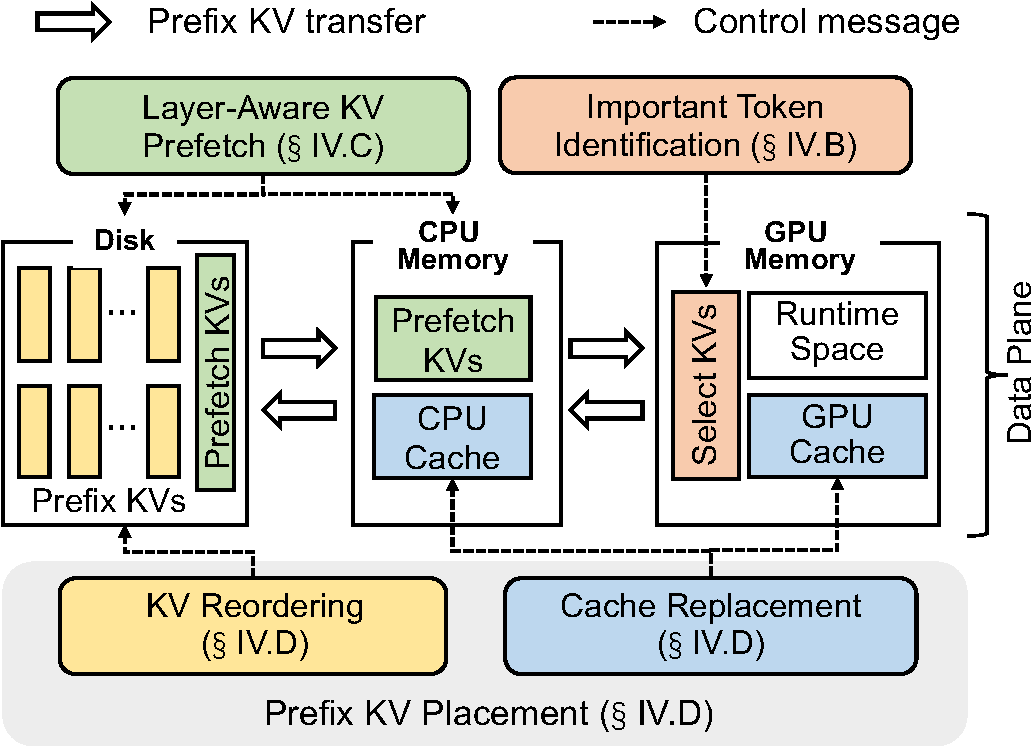
\includegraphics[width=3.3in]{overview.pdf}
	\caption{\cp{Overview of the \pname{} system.}}
	\label{fig:overview}
	\vspace{-0.2in}
\end{figure}


\noindent \textbf{Dataflow of \pname{}.} 
Assume that a request $S=[t^p_0, t^p_1,...,t^p_{m-1}, t^q_0, t^q_1,...,t^q_{n-1}]$ arrives.
$m$ is the number of tokens in prefix and $n$ is the number of tokens in the query.
$t^p$ and $t^q$ denote the prefix and non-prefix tokens respectively. 
First, given the request, \pname{} searches the radix tree to find the longest common 
prefix subsequence from all previous requests~\cite{sglang-arxiv23, chunkattention-arxiv24}. 
Let's assume the result is  
%$R=[t^p_{i}, t^p_{i+1}, ..., t^p_j]$, whose KVs are 
$R=[t^p_0, t^p_1, ..., t^p_j]$, whose KVs are
stored in GPU memory, CPU memory, or disk.
There may also be some prefix tokens \( NR = [t^p_{j+1}, ..., t^p_{m-1}] \) that are not in the radix tree, and therefore their KVs do not exist in the system.
Next, \pname{} employs the I/O-efficient ITF method to identify 
the important tokens within $R$ , assuming $R_{important}=[t^p_{t}, t^p_{t+1}, ..., t^p_s]$ 
%($ i \leq t \leq s \leq j$) is identified. 
($ 0 \leq t \leq s \leq j$) is identified.
If KVs in $R_{important}$ are not in GPU memory, they are loaded from disk or CPU memory. 
The KVs of unimportant tokens in $R$ are not reused and do not participate in further inference.
Then, the loaded $R_{important}$, the tokens $NR$, and the tokens $[t^q_0, t^q_1,...,t^q_{n-1}]$   
are sent into LLM model, completing the remaining computations in the prefill phase.
Essentially, $R_{important}$ plus $NR$ becomes the defacto prefix used in the LLM inference,
replacing the set of \{$t^p$\} in $S$.
%Finally, the newly generated KVs for the prefix token in $R_{important}$ are stored on disk, 
%and the prefix tokens in $R_{important}$ are inserted into the radix tree for future reuse by other requests. 
Finally, the newly generated KVs for the prefix token in $NR$ are stored on disk, 
and the prefix tokens in $NR$ are inserted into the radix tree for future reuse by other requests. 
The decoding phase remains unchanged, following existing systems~\cite{alluneed-nips17}.

% \wj{
\noindent \textbf{Importance metric.} 
In this paper, we use the sum of values
in each column of the attention weight matrix as the token's importance,
following the same method in H2O~\cite{h2o-nips23}. A higher sum indicates greater
token importance. Our system is also compatible with other metrics for measuring
token importance~\cite{scissorhands-nips23, flexgen-icml23, infinigen-osdi24}.
% }

%\pname{} uses a radix-tree~\cite{sglang-arxiv23} 
%to manage the mapping from a token ID to its location.
%When a user request arrives, it searches the radix tree
%to identify its prefixes shared with previous requests. 
%For each token in the prefix, we design different
%dataflows depending on whether the token
%is an important token. 
%(1) If a token is an important token and exists
%in the radix-tree, its prefix KV will be moved
%to GPU if it does not exist in GPU.
%(2) If a token is an important token but does not
%exist in the radix-tree, its prefix KV will be
%generated through the prefill computation and decoding
%(illustrated in Section 2.1). After that, it is moved to GPU.
%(3) If a token is not an important token, \pname{}
%will substitue its KV with the KV of one important token 
%identified by ITF in the subsequent inference to
%reduce the amount of data for loading/generating 
%prefix KVs.

%\wj{
%When a user request arrives, it searches the radix tree 
%to identify its shared prefixes with previous requests. 
%For each token in the prefix, we design different 
%dataflows depending on whether the token is shared.
%(1) If a token is not shared, its prefix KV will be 
%generated through the prefill computation (illustrated in \cref{sec:llm-basic}). 
%Afterward, the token is inserted into the radix tree, 
%and its prefix KV is stored on disk for future reuse by other requests.
%(2) If a token is shared, it will be evaluated by the ITF 
%to determine if it is an important token. 
%If it is important and its prefix KV is not in GPU memory, 
%the prefix KV will be fetched to the GPU for subsequent inference computation. 
%If it is not important, its prefix KV will be not used for current request's computations.
%}


%(1) If the token ID does not exist in the radix-tree,
%indicating no shared prefix is found, \pname{} will
%insert the token into the radix-tree, perform a complete 
%prefill computation, split the computed prefix KVs into fixed chunks, 
%and stores them on disks. The stored prefix KVs are periodically 
%reordered and the relevant metadata are updated. 
%(2) If the token is found in the radix-tree,
%\pname{} will identify the location of important prefix KVs 
%in the multi-tier storage and move them to GPUs for
%further inference.
%(3) If a subset of tokens are found in radix-tree, indicating
%the current request has a partially shared prefix with
%previous requests, the system will first identify important
%KVs shared among the heads for the current query through ITF.
%Then, for the important KVs exist in the storage, they
%will be moved to GPU. For the remaining, they will be generated
%through prefill computation, along with all subsequent decoding phases 
%in GPUs. The prefix KVs including the newly generated KVs will be either 
%cached in GPU or CPU memory, or discarded (with a copy always retained on 
%disks). Their corresponding metadata are updated accordingly.


%\subsection{Insights of Important Tokens}
%\label{sec:insight}
% Empirical 
%\begin{figure}
%	\centering
%	\subfigure[Two Heads of K Tensors]{
%		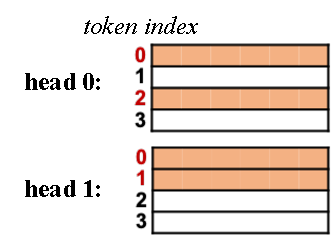
\includegraphics[width=1.5in, height=1in]{jcd-example.pdf}
%		\label{fig:jcd-example}
%	}
%	\hspace{0.06in}
%	\subfigure[Jaccard Scores Between Heads]{
%		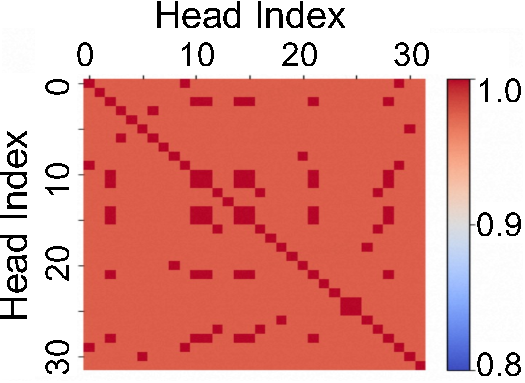
\includegraphics[width=1.5in, height=1in]{real-jcd-example.pdf}
%		\label{fig:real-jcd-example}
%	}
%	\vspace{-0.1in}
%	\caption{Examples of similarities. (a) The orange rows represent the important keys whose token indices are marked in red. (b) Darker squares indicate a higher similarity between the important token index sets of two heads.}
%	\vspace{-0.1in}
%\end{figure}
%
%
%
%%We highlight two key observations regarding the characteristics of important tokens.
%%Although we cannot strictly prove these observations mathematically for all LLMs and scenarios, we demonstrate the generality and practicality of these findings by showing the impact on accuracy when designs based on these observations are applied, across x datasets and x models.
%%, we will demonstrate the generality and practicality of these observations through accuracy evaluations after applying the corresponding techniques on x datasets and x models.
%
%%\vspace{-1.0ex}
%%\begin{framed}
%%\vspace{-1.4ex}
%%\noindent
%%\textbf{Observation I:}{
%%There is a high similarity in the set of important token indices 
%%across different heads within the same layer of an LLM.
%%}
%%\vspace{-1.4ex}
%%\end{framed}
%\noindent
%\textbf{Observation I:}{
%	There is a high similarity in the set of important token indices 
%	across different heads within the same layer of an LLM.
%}
%
%%\textbf{Observation 1.} \textit{There is a high similarity in the set of important token indices across different heads within the same layer.}
%
%As described in \cref{sec:llm-basic}, each token has K and V tensors for every head. We found that the set of important token indices is highly similar across different heads within the same layer. This is intuitive because the \( k\) or \( v \) tensors in different heads are derived from the same large K or V tensors~\cite{alluneed-nips17, opt-arxiv22}. Therefore, if a token is significantly more important than another in one head, it is highly likely that this importance relationship holds in other heads as well. Note that although we cannot strictly prove these observations mathematically for all LLMs and scenarios, we will demonstrate the generality and practicality of these observations through accuracy evaluations (\cref{exp:overall}) after applying the corresponding techniques on four datasets across three models.
%
%To quantitatively measure the similarity between these index sets, we use the Jaccard index~\cite{jaccard-18}. Assume the sets of the most important token indices selected from two heads are A and B. The jaccard index is defined as the size of the intersection divided by the size of the union of the two sets: \( J(A, B) = \frac{|A \cap B|}{|A \cup B|} \). The Jaccard value is 0 when the two important token index sets are completely different and 1 when they are identical.
%Figure~\ref{fig:jcd-example} shows an example where an input sequence contains four tokens, of which 50\%  are considered as important tokens. The index set of important tokens for the keys of head 0 is  \( h_0 = \{0, 2\} \), and for head 1 it is \( h_1 = \{0, 1\} \). The similarity between the important token indices in these two heads is \( J(h_0, h_1) = \frac{|h_0 \cap h_1|}{|h_0 \cup h_1|} = \frac{1}{3} \).
%Figure~\ref{fig:real-jcd-example} shows a real similarity heatmap of the important token sets in the keys produced by the middle transformer layer of the OPT-6.7B model. It demonstrates that these similarities are quite high, with average values exceeding 0.95. 
%
%\begin{figure}
%	\centering
%	\subfigure[select the top 10\% most important tokens]{
%		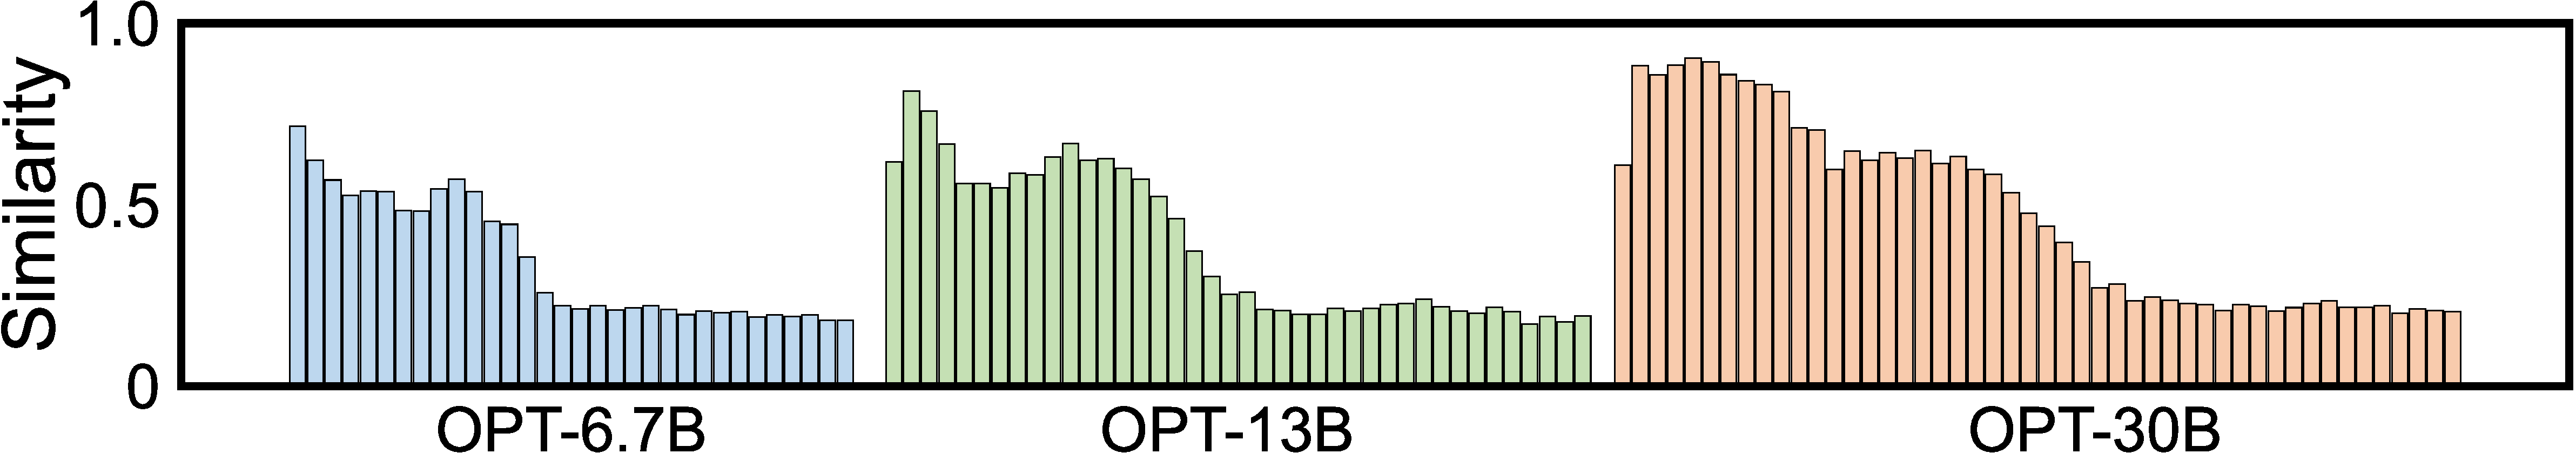
\includegraphics[width=3.2in, height=0.6in]{sim-ten.pdf}
%	}
%	\subfigure[select the top 40\% most important tokens]{
%		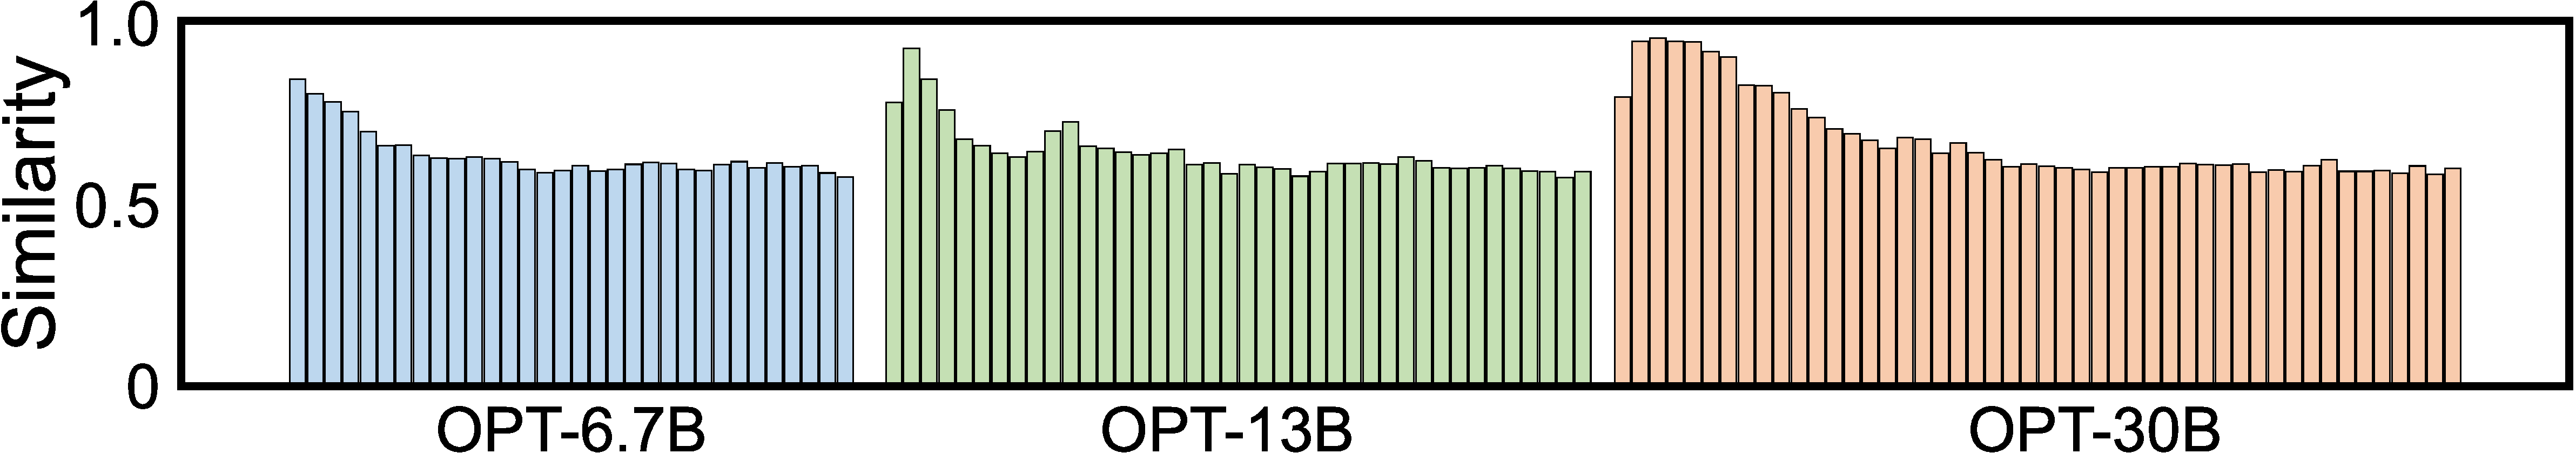
\includegraphics[width=3.2in, height=0.6in]{sim-forty.pdf}
%	}
%	\vspace{-0.1in}
%	\caption{Similarities of important token index sets across all transformer layers.}
%	\label{fig:simi-values}
%	\vspace{-0.1in}
%\end{figure}
%
%%This observation holds across different sampling ratios and LLM scales.
%%For example, Figure~\ref{} shows that as the proportion of important tokens selected varies from 10\% to 100\%, the average similarity across all layers of the OPT-30B model exceeds xx for a randomly selected request from the xx dataset. Figure~\ref{} shows that the average similarity across all layers of the OPT models, ranging from 1.3B to 30B, is consistently greater than x.
%%when the proportion of important tokens is set to xx, 
%
%%\vspace{-1.0ex}
%%\begin{framed}
%%\vspace{-1.2ex}
%%\noindent
%%\textbf{Observation II:}{
%%The similarity of important tokens (represented as important token index sets) exists across different sampling ratios and LLM scales.
%%}
%%\end{framed}
%\noindent
%\textbf{Observation II:}{
%	The similarity of important tokens (represented as important token index sets) exists across different sampling ratios and LLM scales.
%}
%
%To gain further insights, we study the average similarity of token index sets across different heads for the OPT-6.7B, OPT-13B, and OPT-30B models,
%%\ysl{This analysis focuses on scenarios where the top 10\% and 40\% of the most critical tokens were selected, as illustrated in Figure~\ref{fig:simi-values}.}
%when selecting the top 10\% and 40\%  most important tokens (Figure~\ref{fig:simi-values}). 
%Each bar in the figure represents the average value for a single transformer
%layer. These three models contain a total of 32, 40, and 48 transformer layers,
%respectively. We have two findings.
%(1) The higher ratio of important tokens selected, the greater the similarity. For instance, when selecting 40\% and 10\% of the tokens, the average similarity across all layers of OPT-30B is 0.68 and 0.48, respectively. This aligns with intuition, as the similarity reaches 1 when all the tokens (100\%) are selected. 
%(2) Although smaller models and deeper transformer layers tend to exhibit lower similarities, they are still significantly higher than the expected value from random selection in most cases. 
%%For example, while the last layer of OPT-6.7B has a similarity value of only 0.18 when selecting the top 10\% important tokens, the expected similarity from randomly selecting 10\% of tokens is merely \( 10\% / (2 - 10\%) \approx 0.053 \). 
%%This indicates that the observation does indeed hold across different models and layers, even if it is sometimes less pronounced.
%%(2) Larger models tend to exhibit higher similarity. For example, when selecting 50\% of the tokens, the average similarity across all layers of OPT-30B and OPT-6.7B is xx and yy, respectively. This could be attributed to the stronger inference capabilities of larger models, which result in more distinct differences between the vector representations of important and unimportant tokens, leading to more consistent important token index sets across different heads.
%%(3) Within the same model, deeper transformer layers tend to have lower similarity compared to shallower ones. This may be because shallower transformer layers focus on extracting specific features from tokens, while deeper blocks capture more complex relationships between tokens, causing greater variation in the important tokens identified by different heads.
%
%
%
%%\textbf{Observation 2:} \textit{.}
%\noindent
%\zrdnew{
%\textbf{Observation III: }
%{Important token indices also exhibit strong consistency across adjacent layers of an LLM}
%}
%
%xxx

\subsection{\techA{}}

\label{sec:techa}

\begin{figure}
	\centering
	\subfigure[Two Heads of K Tensors]{
		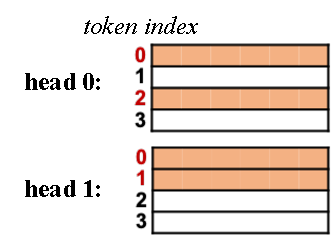
\includegraphics[width=1.5in, height=1in]{jcd-example.pdf}
		\label{fig:jcd-example}
	}
	\hspace{0.06in}
	\subfigure[Jaccard Scores Between Heads]{
		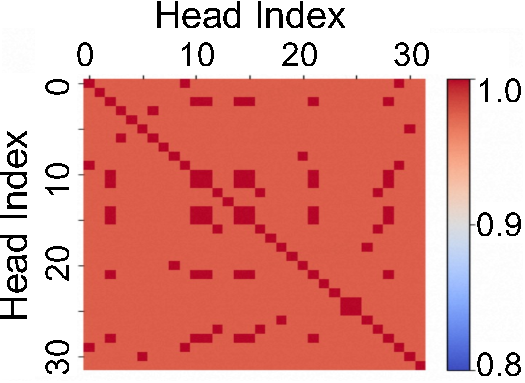
\includegraphics[width=1.5in, height=1in]{real-jcd-example.pdf}
		\label{fig:real-jcd-example}
	}
	\vspace{-0.1in}
	\caption{Examples of similarities. (a) The orange rows represent the important keys whose token indices are marked in red. (b) Darker squares indicate a higher similarity between the important token index sets of two heads.}
	\vspace{-0.1in}
\end{figure}



%We highlight two key observations regarding the characteristics of important tokens.
%Although we cannot strictly prove these observations mathematically for all LLMs and scenarios, we demonstrate the generality and practicality of these findings by showing the impact on accuracy when designs based on these observations are applied, across x datasets and x models.
%, we will demonstrate the generality and practicality of these observations through accuracy evaluations after applying the corresponding techniques on x datasets and x models.

%\vspace{-1.0ex}
%\begin{framed}
%\vspace{-1.4ex}
%\noindent
%\textbf{Observation I:}{
	%There is a high similarity in the set of important token indices 
	%across different heads within the same layer of an LLM.
	%}
%\vspace{-1.4ex}
%\end{framed}
\noindent
\textbf{Observation I:}{
	There is a high similarity in the set of important token indices 
	across different heads within the same layer of an LLM.
}

%\textbf{Observation 1.} \textit{There is a high similarity in the set of important token indices across different heads within the same layer.}

As discussed in \cref{sec:llm-basic}, each token has K and V tensors for every head. 
We observe that important token indices are highly similar across heads within the same layer, 
as \(k\) and \(v\) tensors originate from the same large K and V tensors~\cite{alluneed-nips17, opt-arxiv22}. 
Thus, a token important in one head is likely important in others. 
While this cannot be formally proven for all LLMs, its generality and practicality are validated through accuracy evaluations (\cref{exp:overall}) on four datasets across three models.


To quantify the similarity between important token index sets, we use the Jaccard index~\cite{jaccard-18}, defined as 
\( J(A, B) = \frac{|A \cap B|}{|A \cup B|} \),
where \(A\) and \(B\) denote the important token index sets of two heads. 
The value ranges from 0 (completely different) to 1 (identical). 
As shown in Figure~\ref{fig:jcd-example}, for an input with four tokens where 50\% are important, 
\( h_0 = \{0, 2\} \) and \( h_1 = \{0, 1\} \), yielding \( J(h_0, h_1) = \frac{1}{3} \). 
A real similarity heatmap from the middle layer of OPT-6.7B (Figure~\ref{fig:real-jcd-example}) 
shows high similarity among heads, with average values exceeding 0.95.


\begin{figure}
	\centering
	\subfigure[select the top 10\% most important tokens]{
		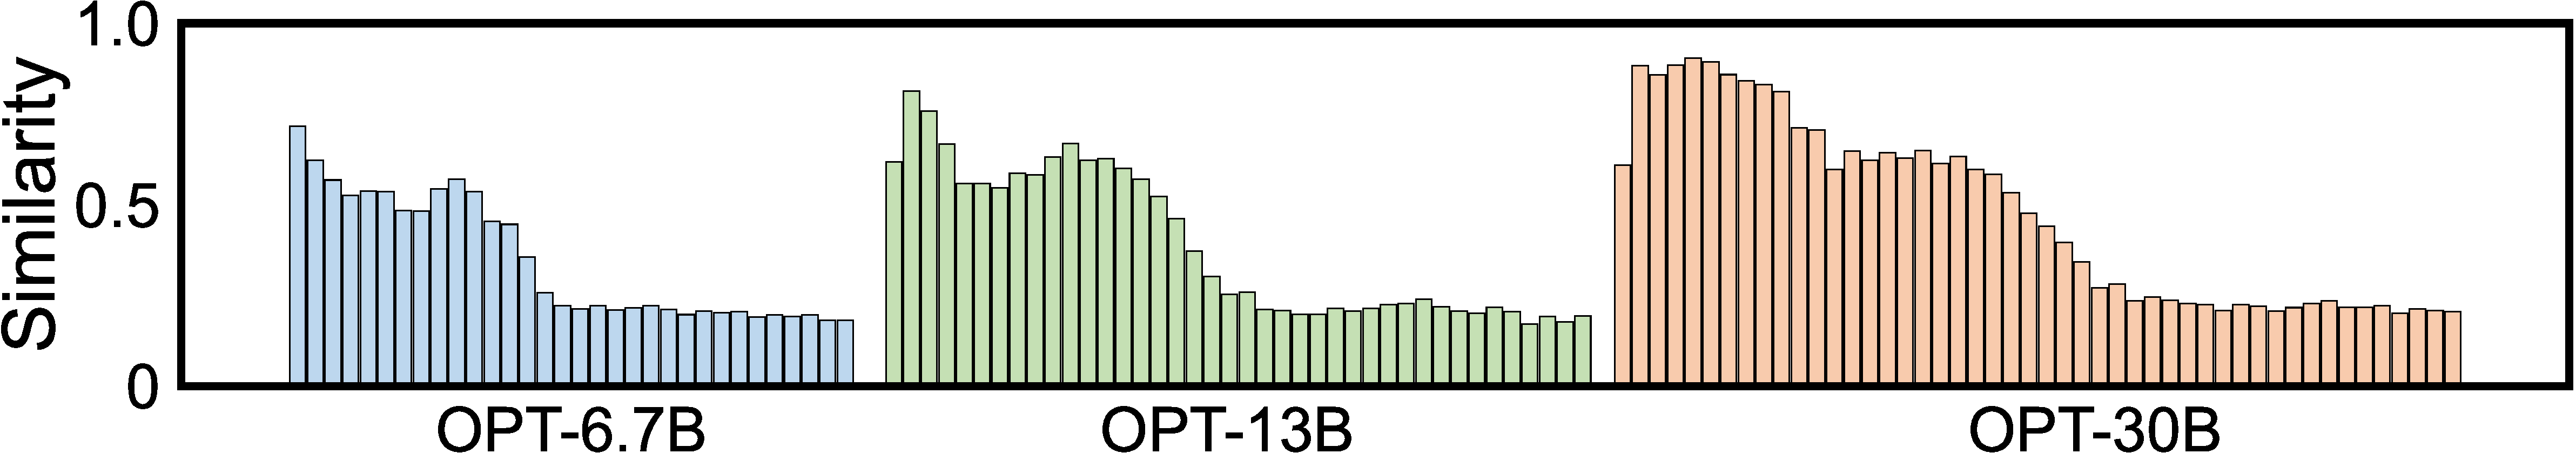
\includegraphics[width=3.2in, height=0.6in]{sim-ten.pdf}
	}
	\subfigure[select the top 40\% most important tokens]{
		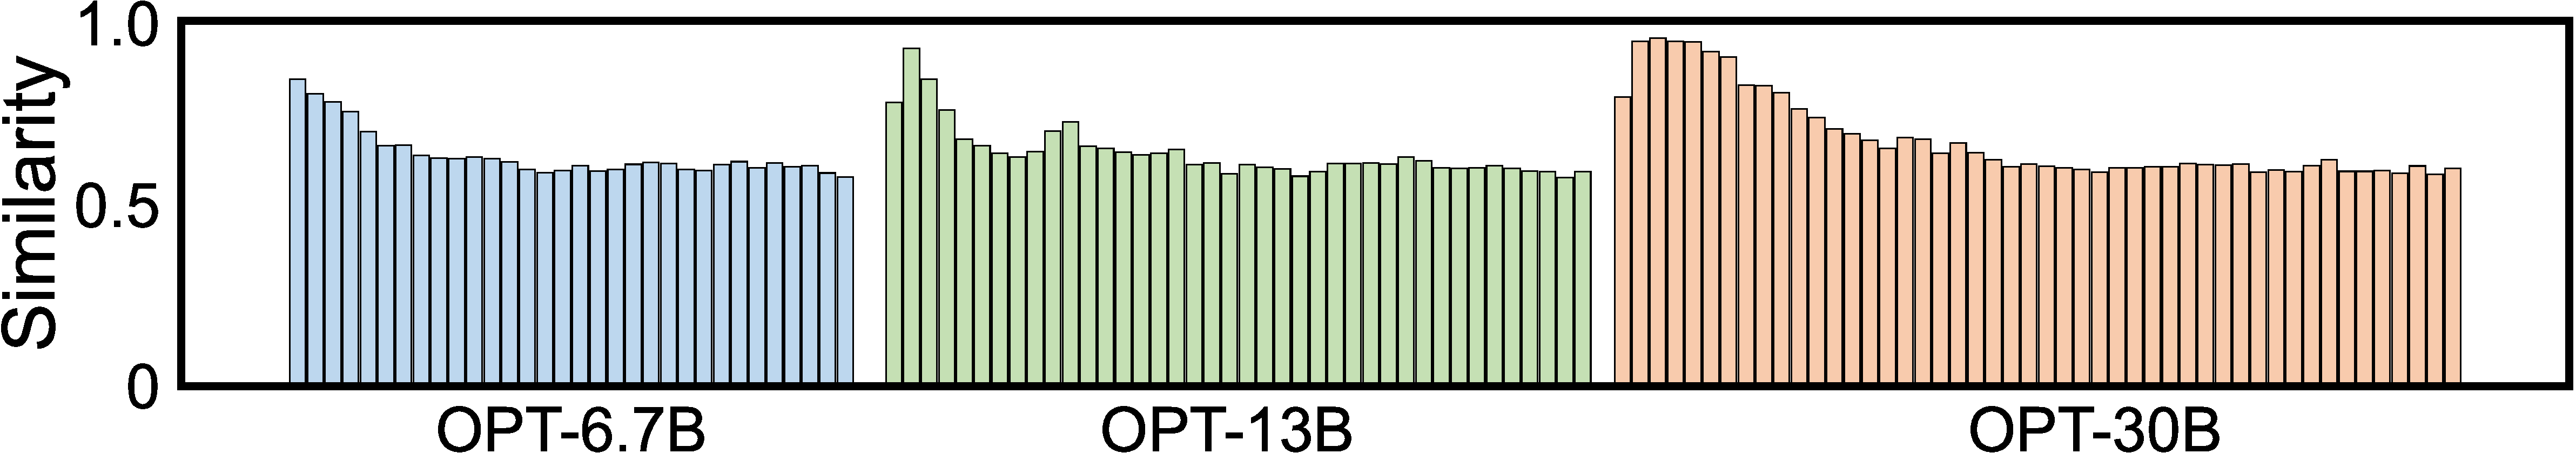
\includegraphics[width=3.2in, height=0.6in]{sim-forty.pdf}
	}
	\vspace{-0.1in}
	\caption{Similarities of important token index sets across all transformer layers.}
	\label{fig:simi-values}
	\vspace{-0.1in}
\end{figure}

%This observation holds across different sampling ratios and LLM scales.
%For example, Figure~\ref{} shows that as the proportion of important tokens selected varies from 10\% to 100\%, the average similarity across all layers of the OPT-30B model exceeds xx for a randomly selected request from the xx dataset. Figure~\ref{} shows that the average similarity across all layers of the OPT models, ranging from 1.3B to 30B, is consistently greater than x.
%when the proportion of important tokens is set to xx, 

%\vspace{-1.0ex}
%\begin{framed}
%\vspace{-1.2ex}
%\noindent
%\textbf{Observation II:}{
	%The similarity of important tokens (represented as important token index sets) exists across different sampling ratios and LLM scales.
	%}
%\end{framed}
\noindent
\textbf{Observation II:}{
	The similarity of important tokens (represented as important token index sets) exists across different sampling ratios and LLM scales.
}

To further understand this phenomenon, we analyze the average similarity of important token index sets across different heads for the OPT-6.7B, OPT-13B, and OPT-30B models when selecting the top 10\% and 40\% most important tokens (Figure~\ref{fig:simi-values}). 
Each bar denotes the average similarity for one transformer layer, with 32, 40, and 48 layers in the three models, respectively. 
We have two findings: 
(1) selecting a larger proportion of important tokens leads to higher similarity. For example, in OPT-30B, the average similarity is 0.68 when selecting 40\% tokens and 0.48 when selecting 10\%, consistent with the intuition that similarity approaches 1 when all tokens are included; 
(2) although smaller models and deeper layers generally show lower similarity, they remain substantially above the random-selection baseline in most cases.

%For example, while the last layer of OPT-6.7B has a similarity value of only 0.18 when selecting the top 10\% important tokens, the expected similarity from randomly selecting 10\% of tokens is merely \( 10\% / (2 - 10\%) \approx 0.053 \). 
%This indicates that the observation does indeed hold across different models and layers, even if it is sometimes less pronounced.
%(2) Larger models tend to exhibit higher similarity. For example, when selecting 50\% of the tokens, the average similarity across all layers of OPT-30B and OPT-6.7B is xx and yy, respectively. This could be attributed to the stronger inference capabilities of larger models, which result in more distinct differences between the vector representations of important and unimportant tokens, leading to more consistent important token index sets across different heads.
%(3) Within the same model, deeper transformer layers tend to have lower similarity compared to shallower ones. This may be because shallower transformer layers focus on extracting specific features from tokens, while deeper blocks capture more complex relationships between tokens, causing greater variation in the important tokens identified by different heads.



%\textbf{Observation 2:} \textit{.}

\textbf{Design}. Based on the above observations, we propose the \techa{} technique. The core idea is that \textit{because of the similarity we can leverage the important token index set generated from a few selected heads to approximate the important token index sets for the remaining heads}. For simplicity, we refer to these selected heads as \textit{probe heads}. Since this process involves loading only keys from a subset of the heads instead of all heads, it reduces both I/O data volume and TTFT.

As some layers exhibit less pronounced similarity between important token
sets across different heads, applying this technique to these layers may
misidentify important tokens in some heads, reducing the model's
inference accuracy. To tackle this issue, we introduce a similarity threshold
that dynamically determines whether to apply the technique
for each transformer layer.
The \techa{} is enabled only when the measured similarity value from the probe heads 
is higher than the similarity threshold.

\begin{figure}
	\centering
	\subfigure[w/o similarity-guided token selection]{
		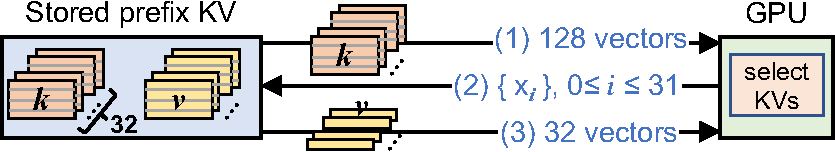
\includegraphics[width=3.2in, height=0.6in]{wo-techa.pdf}
	}
	\subfigure[w/ similarity-guided token selection]{
		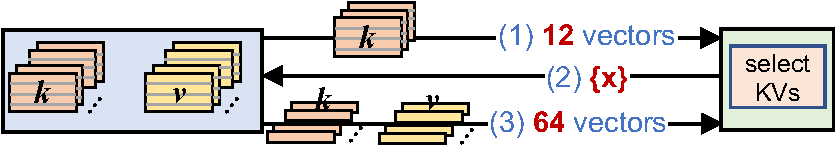
\includegraphics[width=3.2in, height=0.6in]{w-techa.pdf}
	}
	\vspace{-0.1in}
	\caption{The process of transformer layer computation with prefix kv. Each \(k\) and \(v\) tensor has four row vectors because of four tokens in the prefix.}
	\label{fig:woandw-techa}
	\vspace{-0.1in}
\end{figure}



\zrd{Figure~\ref{fig:woandw-techa} illustrates the process of completing a transformer layer with and without this technique. Assume the prefix contains 4 tokens, with only one being important. Each transformer layer has 32 heads and all the prefix KVs of each head are stored on disk. The number of probe heads is set to three. 
Without it, all 32 heads must load 128 key vectors and later 32 \(k,v\) vectors, totaling 160 vectors. 
With \techa{}, only 12 key vectors from three probe heads are first loaded. The GPU computes attention and measures probe-head similarity. 
If the similarity exceeds the threshold, only one token index deemed most important by all probe heads \(\{x\}\) is used, and 64 \(k,v\) vectors are loaded---just 76 vectors in total. 
When the threshold is unmet, the process reverts to the standard mode, though this occurs in fewer than 20\% of layers. 
Given that modern LLMs have dozens of heads and long prefixes, \techa{} effectively reduces I/O load across most layers. }
%Figure~\ref{fig:woandw-techa} illustrates the process of completing a transformer layer with and without this technique. Assume the prefix contains 4 tokens, with only one being important. Each transformer layer has 32 heads and all the prefix KVs of each head are stored on disk. The number of probe heads is set to three. 
%Without the \techa{} technique, it involves three steps: 
%(1) loading the keys of all 32 heads (total 32 $\times$ 4 = 128 vectors) from
%disk into the GPU memory; 
%(2) GPU calculates attention weights using the query and all the keys,
%identifies the most important token index in each head \( i \): $\{x_i\}, \ 0
%\leq i \leq 31$, and returns them to the CPU memory; The detailed identification
%algorithm is based on H2O~\cite{h2o-nips23}.
%(3) The CPU then loads the \(k\) and \(v\) vectors of $\{x_i\}$ from each head
%(total 32 $\times$ 1 = 32 vectors) into the GPU memory to complete the remaining
%prefill computations. The entire process loads a total of 128 + 32 = 160
%vectors.
%
%In contrast, with the \techa{} technique, the steps are as follows:
%(1) only the keys from the three probe heads (total 3 $\times$ 4 = 12 vectors)
%are loaded from disk into the GPU memory; 
%(2) GPU calculates attention weights using the query and the keys from the probe heads, 
%identifies the important token index sets of the three heads, 
%and computes the average Jaccard similarity. 
%If this similarity exceeds the similarity threshold, only one token index 
%deemed most important by all probe heads, $\{x\}$, are returned to the CPU; Then, proceed to step (3).
%If the threshold is not met, the computation mode of the current layer falls back to the version without enabling the \techa{} method.
%(3) The CPU then loads the \(k\) and \(v\) vectors of $\{x\}$ from each head
%(total 32 $\times$ 1 $\times$ 2 = 64 vectors) into the GPU  memory for the remaining
%computations. The entire process loads a total of 12 + 64 = 76 vectors.
%While the I/O data volume cannot be reduced when the probe heads' similarity does not exceed the threshold, this situation only occurs in less than 20\% transformer layers in the \pname{} system on average (see \cref{exp:indiv}). Moreover, in practical LLM models, each transformer layer typically has dozens of heads (e.g., 32-96 in various sizes of the OPT model) and the prefix contains thousands of tokens~\cite{chunkattention-arxiv24, cachegen-sigcomm24}, making this technique effective in reducing I/O data volume across the entire model.
%

\begin{figure}
	\centering
	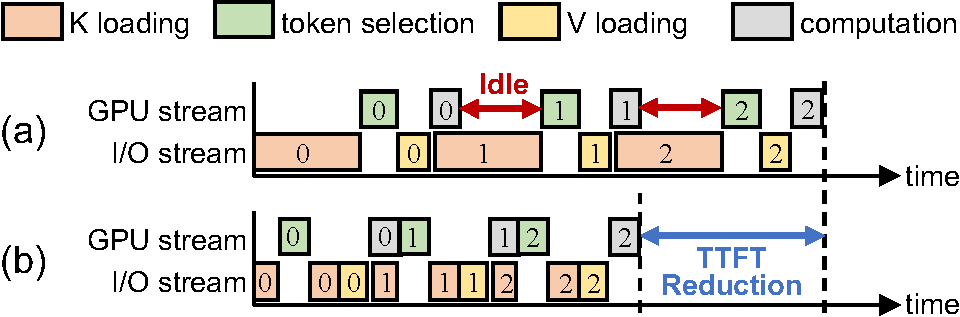
\includegraphics[width=3.4in, height=1.2in]{simiload-ttft.pdf}
	\caption{The TTFTs with and without \techa{}. Assume the LLM model consists of three transformer layers. The numbers inside the rectangles represent the layer index.}
	\label{fig:simiload-ttft}
\end{figure}


Figure~\ref{fig:simiload-ttft} compares the timeline for completing three transformer layers with and without this technique. 
Without \techa{}, in Figure~\ref{fig:simiload-ttft}(a), the loading of a large number of keys leads to GPU idle time, prolonging inference process. In contrast, when the technique is enabled in Figure~\ref{fig:simiload-ttft}(b), and the probe heads’ similarity exceeds the threshold, the time required to load only the keys from the probe heads (in red color) is significantly shorter, thereby reducing GPU wait time. Additionally, loading only a subset of keys for attention weight calculations reduces the time spent generating important token index sets (in green color), leading to a shorter overall TTFT.

\noindent \textbf{Hyperparameter decisions.}
%To make this algorithm practical, we need to determine the number of probe heads and the similarity threshold.
%Selecting only one probe head to determine the most important token index may introduce bias, affecting model accuracy. Using two probe heads might fail to identify the most important index through voting when disagreements arise. Therefore, we choose to use three probe heads. Increasing the number of probe heads offers minimal improvements in accuracy but increases the keys loading time, thereby extending the TTFT.
%Additionally, we found that the choice of which three heads to use has no impact on accuracy due to the similarity. 
%Therefore, we simply select the first three heads in each transformer layer as the probe heads to keep the selection process quick.
%\fv{
%We first compute the similarity of important token sets between each pair of  probe heads, and then take the average to measure the overall similarity among the three probe heads. Thus, the similarity is independent of the order of probe heads.
%}
\zrd{To make the algorithm practical, we need to determine the number of probe heads and the similarity threshold. Using a single probe head may introduce bias, while two heads can yield inconsistent voting results. We therefore adopt three probe heads, which balance accuracy and efficiency. Adding more heads provides negligible accuracy gains but increases key-loading latency and TTFT. Since the choice of heads has minimal effect due to their high similarity, we simply use the first three heads in each transformer layer for fast selection. 
}


\begin{figure}
	\centering
	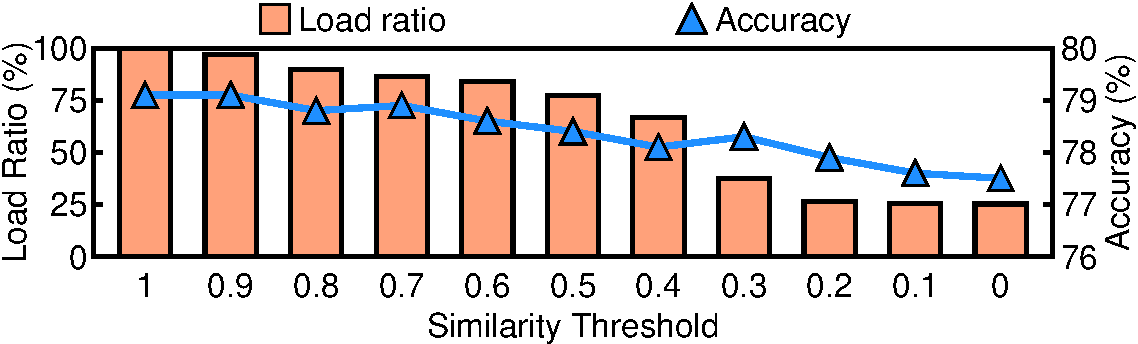
\includegraphics[width=3.3in, height=1in]{dif_sim_thred.pdf}
	\vspace{-0.1in}
	\caption{
		The proportion of keys loaded and the model inference accuracy under different similarity thresholds.}
	\label{fig:thred}
	\vspace{-0.1in}
\end{figure}


% Determining the similarity threshold is not trivial. A threshold that is too high may result in not reducing the number of keys and values in many transformer layers because the average similarity of the probe heads is consistently below the threshold. Conversely, a threshold that is too low can lead to biased results in the identified important token index set, thereby degrading model accuracy. 
% Figure~\ref{fig:thred} shows an example on the PIQA~\cite{lmeval} dataset, where we set each transformer layer to select 25\% of the most important prefix KVs. Although lowering the threshold from 1 to 0 reduces the number of keys loaded by 4$\times$, it also causes a drop in accuracy from 79.1\% to 77.5\%.
% Similar trends are observed on other datasets.

%Setting the similarity threshold is complex. A threshold set too high might fail to reduce the number of keys and values across many transformer layers, as the average similarity of the probe heads often falls short of the threshold. On the other hand, a threshold set too low can introduce bias in the identified important token index set, compromising model accuracy.
%Figure~\ref{fig:thred} illustrates this on the PIQA~\cite{lmeval} dataset, where each transformer layer selects the top 25\% of the most critical prefix KVs. Although decreasing the threshold from 1 to 0 cuts the number of keys loaded by 4$\times$, it also results in a 1.6\% decrease in accuracy, from 79.1\% to 77.5\%. Similar patterns are observed across other datasets.
%
%
%To address this issue, we first calculate the expected value based on the proportion of selected important tokens, then slightly increase this value and use it as the similarity threshold.
%Specifically, suppose we have a prefix containing \(n\) tokens and need to select \(k\) important tokens (\(k \leq n\)). If we randomly execute this selection twice, we obtain sets \(A\) and \(B\). The probability of each token appearing in both sets is \(\frac{k^2}{n^2}\). Given \(N\) tokens in total, \(E(A \cap B) = n \cdot \frac{k^2}{n^2}\ = \frac{k^2}{n}\), and \(E(A \cup B) = E(A) + E(B) - E(A \cap B) = k + k - \frac{k^2}{n} = 2k - \frac{k^2}{n}\). Therefore, \(E(\text{Jaccard}(A, B)) = \frac{E(A \cap B)}{E(A \cup B)} = \frac{k/n}{2 - (k/n)}\). Denote this expected value as \(j\). We set the threshold \(t = j^\alpha\), where we empirically choose \(\alpha = 0.6\) in our experiments to achieve a good balance between model inference accuracy and the amount of keys loaded. 
\zrd{Setting the similarity threshold requires careful balance. A threshold that is too high prevents key–value reduction across layers, while one that is too low biases the important-token selection and harms accuracy. As shown in Figure \ref{fig:thred} on the PIQA \cite{lmeval} dataset, lowering the threshold from 1 to 0 reduces key loading by 4× but decreases accuracy by 1.6 points (79.1% → 77.5%), with similar trends across other datasets.
To mitigate this, we estimate the expected Jaccard similarity between two random selections of $k$ important tokens from $n$ candidates as $E(\text{Jaccard}) = \frac{k/n}{2 - (k/n)}$, denoted by $j$, and set the threshold to $t = j^{\alpha}$. Empirically, choosing $\alpha = 0.6$ provides a good trade-off between inference accuracy and the number of loaded keys.
\zrd{Setting the similarity threshold is crucial. 
	A high threshold may fail to reduce key-value loading, as probe head similarity often falls below it; 
	a low threshold, however, can bias the selected important tokens and degrade accuracy. 
	As shown in Figure~\ref{fig:thred} on the PIQA~\cite{lmeval} dataset, each transformer layer selects the top 25\% most critical prefix KVs. 
	Lowering the threshold from 1 to 0 reduces the number of loaded keys by 4$\times$, but also decreases accuracy from 79.1\% to 77.5\%. 
	Similar trends hold across other datasets.
}


To address this issue, we first calculate the expected value based on the proportion of selected important tokens, then slightly increase this value and use it as the similarity threshold.
Specifically, suppose we have a prefix containing \(n\) tokens and need to select \(k\) important tokens (\(k \leq n\)). If we randomly execute this selection twice, we obtain sets \(A\) and \(B\). The probability of each token appearing in both sets is \(\frac{k^2}{n^2}\). Given \(N\) tokens in total, \(E(A \cap B) = n \cdot \frac{k^2}{n^2}\ = \frac{k^2}{n}\), and \(E(A \cup B) = E(A) + E(B) - E(A \cap B) = k + k - \frac{k^2}{n} = 2k - \frac{k^2}{n}\). Therefore, \(E(\text{Jaccard}(A, B)) = \frac{E(A \cap B)}{E(A \cup B)} = \frac{k/n}{2 - (k/n)}\). Denote this expected value as \(j\). We set the threshold \(t = j^\alpha\), where we empirically choose \(\alpha = 0.6\) in our experiments to achieve a good balance between model inference accuracy and the amount of keys loaded. 
%\zrd{Setting the similarity threshold requires careful balance. A threshold that is too high prevents key–value reduction across layers, while one that is too low biases the important-token selection and harms accuracy. As shown in Figure \ref{fig\:thred} on the PIQA \cite{lmeval} dataset, lowering the threshold from 1 to 0 reduces key loading by 4× but decreases accuracy by 1.6 points (79.1% → 77.5%), with similar trends across other datasets.
%	To mitigate this, we estimate the expected Jaccard similarity between two random selections of $k$ important tokens from $n$ candidates as $E(\text{Jaccard}) = \frac{k/n}{2 - (k/n)}$, denoted by $j$, and set the threshold to $t = j^{\alpha}$. Empirically, choosing $\alpha = 0.6$ provides a good trade-off between inference accuracy and the number of loaded keys.
%}




%\textbf{\techAa{}}

\subsection{\techNew{}}
\label{sec:techc}
% \subsection{Data Locality in Micrographs}
\label{sec:technew}

%基于
\noindent
\zrdnew{
	\textbf{Observation III: }
	{Important token indices exhibit strong consistency across adjacent layers of an LLM.} To further analyze the distribution of important token indices, we examine the similarity of the top 25\% important token sets across adjacent layers for different models. As shown in Figure~\ref{fig:ob3}(a), there are two key observations: (1) the important tokens exhibit strong consistency across layers, and (2) tokens with higher importance in one layer are more likely to remain important in the subsequent layer.
	Specifically, xxxx.}
% 把图中的一些趋势或者例子挑出来说一下。

%
\begin{figure}
	\centering
	\subfigure[select the top 25\% most important tokens]{
		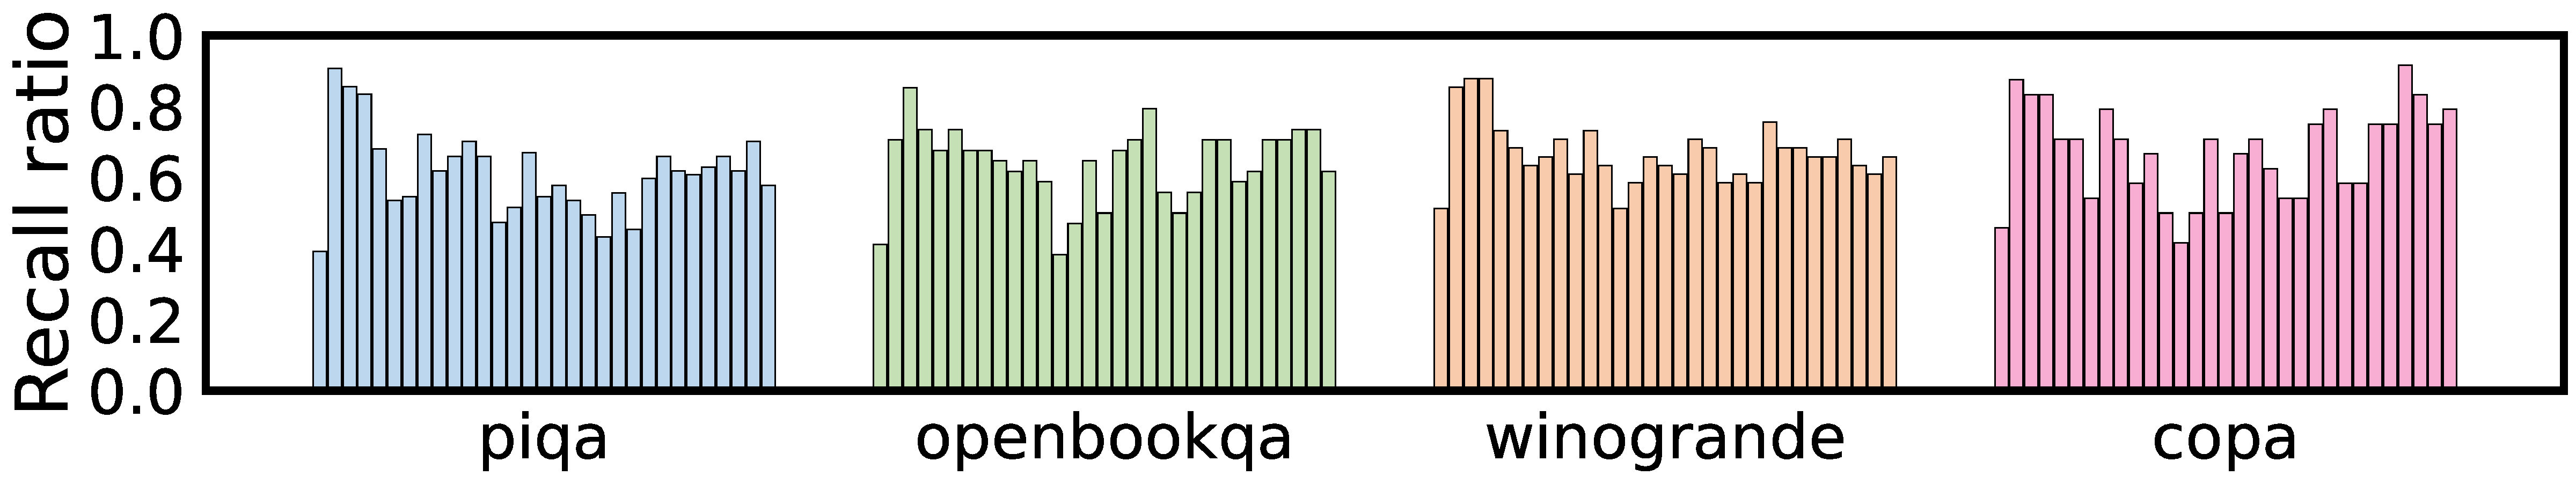
\includegraphics[width=1.5in, height=1in]{sim-25-cross-layers.pdf}
	}
	\subfigure[select different percentage most important tokens]{
		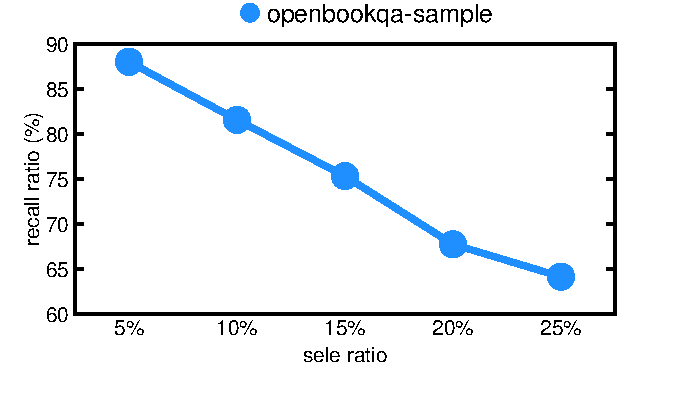
\includegraphics[width=1.5in, height=1in]{recall-sele.pdf}
	}
	\vspace{-0.1in}
	\caption{Similarities of important token index sets of adjacent layers.}
	\label{fig:ob3}
	\vspace{-0.1in}
\end{figure}
%如图xx所示,在模型的一层内,识别重要token index set和加载重要token的kv是有数据依赖的,在没有识别得到重要token index set的情况下,我们无法准确预取下一层所需的重要kv,因此在此层计算时,宝贵的I/O带宽没有被利用,在一个本就I/O瓶颈的场景下。一个naive的方法是,随机的预取一些下一层可能用到的token的kvs到GPU memory中,在下一层的重要token选择完成后,再把不在gpu mem的重要kv load到gpu mem中,然而这样的方法受制于完全不知道下一层重要token index的分布,准确率差,浪费了I/O带宽。一些工作提出了attention sink的概念,即一些特定位置的token在推理过程中总是重要的,如prompt的开头和结尾的几个token,然而,仅预取sink位置的token准确率仍不一定高(一些引用),且存在带宽利用不充分的可能。因此我们提出一种准确率高,灵活的指导预取的方法,高效的预取下一层的重要kv,并将预取与计算overlap起来。我们study了\cref{sec:techa}中提到的识别重要token的方法所识别出的重要token,发现在模型的相邻层重要token的分布是相似的,且重要性排名分位越靠前的index集合,相似度越高。相似度仍用jaccard index量化。
%图片xx描述了基于相似性的重要token识别方法识别出的,图片xx

%\zrdnew{For the important tokens identified as shown in Figure xx, within a given layer of the model, there exists a data dependency between identifying the important token index set and loading the corresponding prefix KVs. Without first identifying the important token index set, we are unable to accurately prefetch the necessary KVs for the next layer. As a result, valuable I/O bandwidth remains underutilized during computation in a scenario that is already constrained by I/O bottlenecks. A naive approach would be to randomly prefetch some potential KVs for the next layer into GPU memory. After the important token selection for the next layer is completed, any important KVs not already in GPU memory can then be loaded into it. However, this approach suffers from the challenge of not knowing the distribution of the important token index set for the next layer, resulting in low accuracy and wasted I/O bandwidth. Some works have proposed the concept of attention sinks, where certain tokens at specific positions, such as the beginning and end of a prompt, are always important during inference. However, prefetching only these sink tokens may still result in low accuracy (some references), and there is a risk of inefficient bandwidth utilization.}
%
%\zrdnew{To address these issues, we propose a more accurate and flexible guidance-based prefetching method that efficiently prefetches important KVs for the next layer while overlapping prefetching with computation. We studied the important tokens identified by the method mentioned in \cref{sec:techa} and found that the distribution of important tokens in adjacent layers is highly similar. Moreover, the index sets with higher importance rankings exhibit higher similarity. This similarity is quantified using the Jaccard index.}

\cp{
Loading important KVs during inference lies on the critical path and thus introduces non-negligible latency, as shown in Figure~\ref{}. 
To alleviate this overhead, we explore using prefetching to hide the I/O cost by overlapping data loading with computation. 
However, this presents a key challenge: the important tokens for the next transformer layer are unknown until the current layer’s computation completes, making it difficult to determine which KVs to prefetch in advance. 
To solve this challenge, based on \textit{Observation~III}, we propose the \technew{} mechanism, which exploits the strong similarity of important token index sets across adjacent layers. 
During the computation of the current layer, \technew{} asynchronously prefetches the important KVs of the next layer into GPU memory by approximating the next layer’s important tokens with those identified in the current layer. 
This layer-aware prefetching effectively reduces I/O latency and achieves higher accuracy than random prefetching.}


Existing LLM serving systems often face high inference latency due to inefficient KV management across GPU, CPU, and disk. 
Only KVs stored in GPU memory can be accessed with low latency, while fetching KVs from CPU or disk introduces substantial delay. 
These data transfers frequently occur on the critical path, causing I/O stalls, bandwidth underutilization, and longer time-to-first-token (TTFT). 


To address these issues, we propose an \textbf{importance-informed key–value (KV) prefetching system} with a \textbf{Dual Budget Strategy (DBS)} that jointly optimizes computation and I/O efficiency across heterogeneous storage tiers. 
Instead of merely overlapping data transfer with computation, our approach dynamically determines \emph{which} KVs to load and \emph{how much} I/O time to allocate to each storage tier within a fixed computation window $T_{\text{comp}}$. 
During each iteration, DBS prioritizes the KVs that yield the greatest accuracy improvement per unit of I/O cost and allocates separate time budgets for disk reads and PCIe transfers, ensuring that prefetching proceeds efficiently without exceeding the computational critical path.

Our system comprises two key components: (1) \textbf{importance-aware token prioritization} and (2) \textbf{dual-stage time budgeting}.  
First, each token is assigned an importance score $v(t)$ derived from its attention weight, while the cost of loading it from storage is estimated as $c(t) = c_{\text{disk}}(t) + c_{\text{pcie}}(t)$.  
We compute the ratio $\text{Density}(t) = v(t)/c(t)$ to evaluate how much benefit each unit of I/O time provides and greedily load tokens with the highest densities.  

Second, DBS partitions the computation time $T_{\text{comp}}$ into a disk I/O budget $T_{\text{disk}} = \rho_{\text{disk}}T_{\text{comp}}$ and a PCIe transfer budget $T_{\text{pcie}} = \rho_{\text{pcie}}T_{\text{comp}}$.  
Data are prefetched in a pipeline from disk to CPU and then to GPU, with dynamic budget adjustment to balance both stages and avoid idle time.  
Cached tokens incur negligible cost, while each disk access amortizes latency across multiple tokens, promoting sequential reads and improving throughput.  

Overall, this design minimizes redundant transfers, maximizes bandwidth utilization, and aligns prefetching time with computation, effectively reducing time-to-first-token (TTFT) without sacrificing inference accuracy.



	
%	Based on observation III, we propose the \technew{} mechanism.
%During the computation of the current layer, we  asynchronously prefetch important KVs of the next layer into GPU memory. This prefetching leverages the similarity of important token index sets across layers to improve prefetching accuracy. By approximating the important token index set of the next layer with the set from the current layer, we increase the accuracy of prefetching, leading to better performance compared to random prefetching. Once the important token index set for the next layer is identified, any important tokens' KVs that were not prefetched are then loaded into GPU memory for inference.


\zrdnew{To minimize inference latency in large language models (LLMs), we propose an importance-informed KV prefetching system that integrates a Dual Budget Strategy (DBS) to balance computation and I/O costs across heterogeneous storage tiers. During inference, key-value (KV) pairs are distributed among GPU, CPU, and disk, and the challenge lies in efficiently transferring the most important KVs to the GPU within a fixed computation time $T_{\text{comp}}$. Our design introduces two synergistic components: (1) **importance-aware token prioritization** and (2) **dual-stage time budgeting**. First, we quantify the importance of each token using the attention-based scores from the current layer and derive its expected value $v(t)$. The cost of loading a token $t$ from its storage location is estimated as $c(t) = c_{\text{disk}}(t) + c_{\text{pcie}}(t)$, where $c_{\text{disk}}(t) = \text{size(chunk)}/B_{\text{disk}}$ and $c_{\text{pcie}}(t) = \text{bytes}(t)/B_{\text{pcie}}$ represent the disk-read and PCIe-transfer times respectively. We then compute the **marginal density** $\text{Density}(t) = v(t)/c(t)$ and greedily select tokens with the highest density, ensuring that each unit of I/O time yields maximal contribution to model accuracy. Second, to achieve precise overlap between I/O and computation, we split the total time budget $T_{\text{comp}}$ into a **disk I/O budget** $T_{\text{disk}} = \rho_{\text{disk}}T_{\text{comp}}$ and a **PCIe transfer budget** $T_{\text{pcie}} = \rho_{\text{pcie}}T_{\text{comp}}$, where $\rho_{\text{disk}}$ and $\rho_{\text{pcie}}$ control the relative proportions of disk and PCIe utilization. Within each iteration, data are prefetched from disk to CPU and from CPU to GPU in a pipelined fashion, and dynamic adjustment of both budgets ensures that neither channel becomes idle or exceeds the computational critical path. Tokens already cached in GPU or CPU memory incur zero or partial cost, while the first access to a disk chunk amortizes the full read latency over multiple tokens, naturally encouraging dense, contiguous I/O. This design reduces redundant transfers, maximizes effective bandwidth, and guarantees that the prefetch time closely matches the computation time. The algorithm runs in $O(N\log N)$ time due to sorting by marginal density, with $O(N)$ space complexity. Ablation experiments compare the proposed DBS with static and random prefetching baselines under varying disk and PCIe bandwidths. Each experiment measures the time-to-first-token (TTFT), inference accuracy, and I/O efficiency. Specifically, we vary $\rho_{\text{disk}}$ and $\rho_{\text{pcie}}$ between 0.2 and 0.8 and evaluate scenarios where disk I/O or PCIe becomes the primary bottleneck. Experimental results demonstrate that DBS achieves up to 2.8× reduction in TTFT with negligible accuracy degradation (<0.2\%), confirming that balanced dual-stage budgeting and marginal density–based selection jointly maximize inference throughput under strict time constraints.}

\subsection{Importance-Informed KV Placement}
\label{sec:techb}

\subsubsection{\techBa{}}
\label{sec:techba}
% We propose the \techba{} technique to address the issue where unimportant KVs within the same chunk are also loaded and cached when retrieving important KVs. The core idea is to increase the density of important KVs within a chunk by reordering and repacking them into new chunks, thereby reducing bandwidth waste during reads. 
% This reordering and repacking process is performed periodically \wj{(e.g., 10 minutes in our settings)}, based on the average importance of each token throughout the cycle.
% The entire process is executed asynchronously, so the time spent does not impact the main I/O path.

% We introduce the \techba{} method to tackle the problem of loading and caching unimportant KVs alongside important ones within the same chunk. The essence is to enhance the concentration of important KVs in a chunk by periodically reordering and consolidating them into new chunks, which minimizes bandwidth wastage during read operations.
% This reorganization and repacking is scheduled at regular intervals (e.g., every 10 minutes in our configuration), aligned with the average importance of each token over the cycle. The entire operation is conducted asynchronously, ensuring that the time invested does not interfere with the primary I/O operations.

We present the \techba{} method to address the unnecessary loading of unimportant KVs during important KV retrieval. By periodically reorganizing and repacking important KVs into denser chunks, this approach optimizes read efficiency and reduces bandwidth waste.
Scheduled at regular intervals (e.g., every 10 minutes), this process is based on the average token importance and operates asynchronously to avoid disrupting the main I/O flow.


\begin{figure}
	\centering
	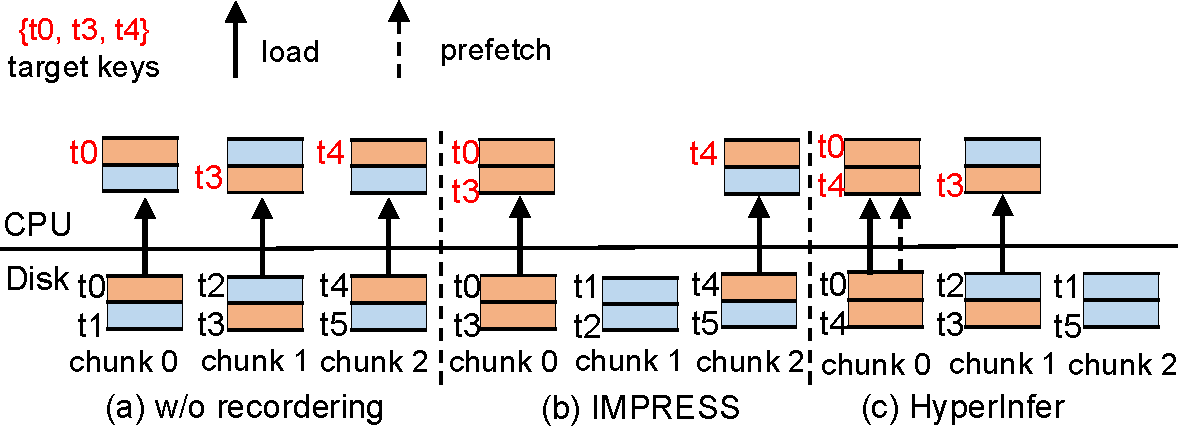
\includegraphics[width=3.4in, height=1.3in]{reorder.pdf}
%	\vspace{-0.1in}
	\caption{Comparison of the number of chunks read before and after the token sequence is reordered. The orange (blue) rectangles represent important (unimportant) keys.}
	\label{fig:reordering}
	\vspace{-0.1in}
\end{figure}

%To illustrate this process, consider an example where a prefix consists of four tokens [t0, t1, t2, t3], and the existing system stores keys for two adjacent tokens in a single chunk. Suppose each chunk contains one important key and one unimportant key.
%Figure~\ref{fig:reordering}(a) demonstrates that, without the \techba{} technique, both chunks must be loaded from disk into CPU memory to retrieve the two important keys \{t0, t3\}. This leads to unimportant keys consuming valuable read bandwidth and cache space. In contrast, with \techba{} enabled (as shown in Figure~\ref{fig:reordering}(b)), the four tokens are first reordered in a descending order of importance, and then the keys of two adjacent reordered tokens (i.e., [t0, t3] and [t1, t2]) are packed into a single chunk. This allows only one chunk to be loaded to access all two important keys, thereby reducing the amount of data read from the disk.
\fvc{
To illustrate, consider a prefix [t0, t1, t2, t3] where the existing system stores keys for two adjacent tokens in one chunk, each containing one important and one unimportant key. Without \techba{} (Figure~\ref{fig:reordering}(a)), both chunks must be loaded to retrieve the important keys \{t0, t3\}, wasting read bandwidth and cache space on unimportant keys. With \techba{} (Figure~\ref{fig:reordering}(b)), tokens are reordered by importance, and keys of adjacent reordered tokens ([t0, t3] and [t1, t2]) are packed into one chunk. This enables loading just one chunk to access all important keys, reducing disk read data.
}

%\noindent \textbf{Metadata adjustment.}
%%In LLM inference, a token's KV can only be reused when that token and all preceding tokens are identical across requests. 
%In LLMs, prefix KVs can only be reused if two prefixes share a common subsequence starting from the first token 
%(i.e., the token order must be the same).
%Therefore, existing systems typically use a radix tree~\cite{sglang-arxiv23, chunkattention-arxiv24} or its variants~\cite{ragcache-arxiv24} to record stored prefix tokens, enabling quick search for reusable stored prefix KVs when a new request arrives. 
%%However, the \techba{} could disrupt the original metadata organization, affecting the ability to check and reuse shared prefix KVs for new requests.
%However, \techba{} may destroy the radix tree structure by altering the token order, 
%causing new requests to fail in locating the correct shared prefix KVs.
%To overcome this, we limit the scope of KV reordering to the tokens within each node of the radix tree. Additionally, we introduce a mapping list within each node to assist the checking operations of new requests.
%We use an example to explain the details.
%
%\begin{figure}
%	\centering
%	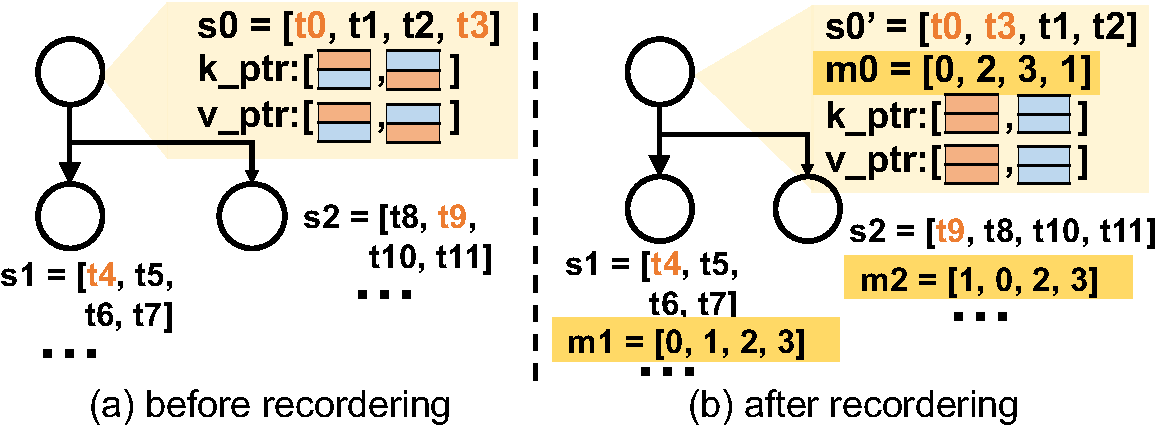
\includegraphics[width=3.3in, height=1.2in]{metaupdate.pdf}
%%	\vspace{-0.1in}
%	\caption{Comparison of meta structure before and after KV reordering. The orange (blue) rectangles represent important (unimportant) keys.}
%	\label{fig:metaupdate}
%	\vspace{-0.1in}
%\end{figure}
%
%Consider two requests that retrieve related document segments as prefixes
%through RAG. Each prefix contains eight tokens: p0=[t0, t1, t2, t3, t4, t5, t6,
%t7] for one request and p1=[t0, t1, t2, t3, t8, t9, t10, t11] for the other. t0,
%t3, t4, and t9 are important data, while the remaining tokens are unimportant.
%Before applying the \techba{} technique, the radix tree is organized as shown in
%Figure~\ref{fig:metaupdate}(a), where the common prefix subsequence s0=[t0, t1,
%t2, t3] is grouped within the same node, enabling the reuse of as many prefix
%KVs as possible. Assume the chunk size is set to 2, with each chunk containing the keys or values of two consecutive tokens.
% Each node contains a list of pointers k\_ptr (v\_ptr) to
%these key (value) chunks.
%
%After enabling \techba{}, as shown in Figure~\ref{fig:metaupdate}(b), the token sequence within each node is reordered in a descending order of importance, and the keys and values are repacked. In Node 0, for example, the token sequence becomes s0' = [t0, t3, t1, t2], with t0 and t3 now grouped within the same chunk. 
%Consequently, reordering disrupts the token sequence in the radix tree.
%We add a new mapping list to Node 0 to address this issue.
%It is denoted as m0 = [0, 2, 3, 1], allowing the original s0 sequence to be recovered using the torch index operation s0'[m0] when search reusable shared prefixes for new requests. This vectorized indexing operation is highly efficient, consuming less than 2\% of the TTFT in our experiments. 
%
%We explicitly avoid cross-node reordering, such as placing t4 and t9 into s0', for two key reasons. First, it would destroy the radix tree structure since t4 and t9 are not common tokens shared by both prefixes (i.e., p0 and p1), potentially leading to errors in retrieving reusable prefix segments for new requests. Second, it would result in unnecessary read bandwidth consumption by loading t9 when reusing the KVs of p0. The constraint against cross-node reordering prevents packing unshared tokens' KVs from different prefixes together, thereby reducing bandwidth wastage.


\subsubsection{\techBb{}}
\label{sec:techbb}
To cut down on PCIe transfers, after loading a chunk from disk into CPU
memory, only the important key and value vectors from that chunk are sent to the
GPU memory via PCIe. However, as depicted in Figure~\ref{fig:imp_token_num}, the
presence of important key or value vectors in a chunk does not align with the
chunk's access frequency. Consequently, existing systems that base their caching
decisions for GPU or CPU memory solely on recency or frequency of chunk access
may lower the GPU cache hit ratio for important key-value pairs, thus increasing
PCIe traffic.

\noindent \textbf{Score-based cache admission.}
To enhance cache efficiency, we introduce the importance-aware cache admission policy.
% \techbb{} policy.
This policy assigns a score to each chunk based on its access frequency and the
proportion of important keys or values it holds. Chunks with higher scores are
preferentially cached in GPU memory, whereas those with lower scores are stored
in CPU memory. This approach boosts the GPU cache hit ratio and minimizes data
transfers between CPU and GPU. The importance ratio is dynamically calculated as
a moving average, updating online after each chunk access.


%\begin{comment}


% For example, assume that key chunk 1 and key chunk 2 come from prefixes requested by application A and application B, respectively, and only one chunk can be stored in the GPU. Since the number of past requests from application A is 1.5 times that of application B, chunk 1 is accessed more frequently than chunk 2. However, only one key (i.e., 50\%) in chunk 1 is important, while both keys (i.e., 100\%) in chunk 2 are important. 
% As shown in Figure~\ref{fig:score_cache}(a), the existing system would place chunk 1 in the GPU and chunk 2 in the CPU because chunk 1 has a higher access frequency. When 15 new requests from application A and 10 new requests from application B arrive, this placement would result in the need to transfer 10 $\times$ 2 = 20 important keys from CPU to GPU. 
% However, considering the importance ratio, chunk 1's score would be 1.5 $\times$ 50\% = 0.75, and chunk 2's score would be 1 $\times$ 100\% = 1. Thus, chunk 2 would be placed in the GPU, as shown in Figure~\ref{fig:score_cache}(b), which would reduce the data transfer during the servicing of the 25 new requests to only 15 $\times$ 1 = 15 important keys.
%\end{comment}

For instance, suppose key chunk 1 from application A and key chunk 2 from
application B are contenders for the limited GPU memory, with application A's
request frequency being 1.5 times that of B, making chunk 1 more frequently
accessed. However, chunk 1 contains only one important key (50\%), while chunk 2
contains two important keys (100\%).
As depicted in Figure~\ref{fig:score_cache}(a), traditional systems would cache
chunk 1 in the GPU memory due to its higher access frequency, relegating chunk 2 to
the CPU. With 15 new requests from A and 10 from B, this approach would
necessitate transferring 20 important keys from CPU to GPU.
By contrast, factoring in the importance ratio, chunk 1 scores 0.75 (1.5 $\times$
50\%), and chunk 2 scores 1 (1 $\times$ 100\%). Thus, our method caches chunk 2 in
the GPU memory, as shown in Figure~\ref{fig:score_cache}(b), cutting the transfer of
important keys to just 15.

\begin{figure}
	\centering
	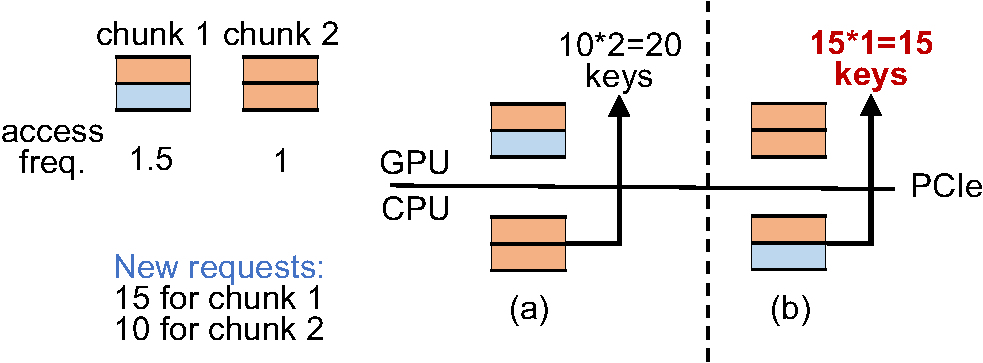
\includegraphics[width=3.3in, height=1.2in]{score_cache.pdf}
	% \vspace{-0.1in}
	\caption{Comparison of two cache replacement policies.(a) is the
	frequency-based cache replacement policy and (b) is the \techbb{} policy. The orange (blue) rectangles
	represent important (unimportant) keys. Only important keys are needed for
	new requests.}
	\label{fig:score_cache}
	\vspace{-0.1in}
\end{figure}


\begin{figure*}
	\subfigure[PIQA]{
		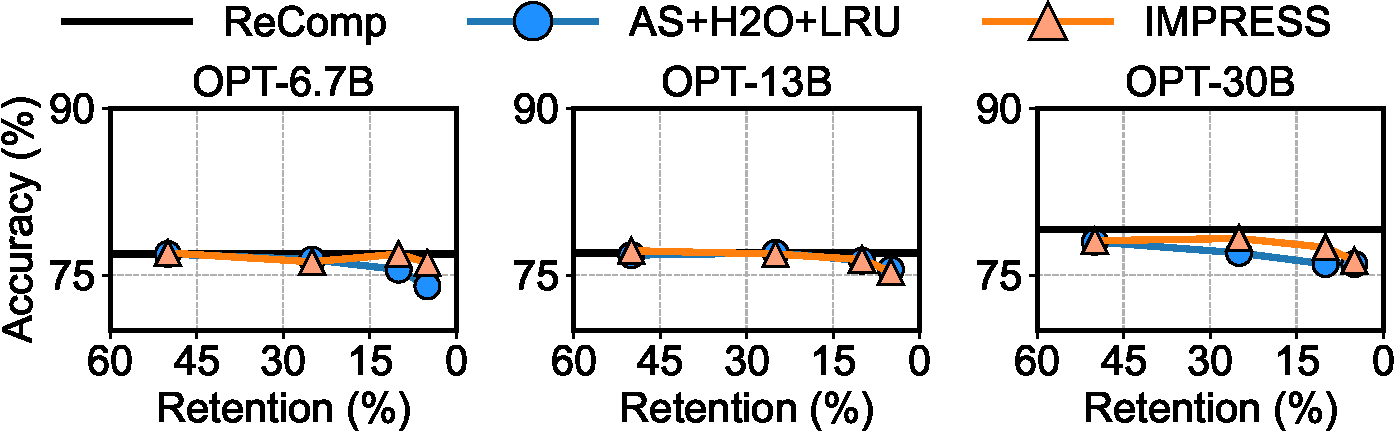
\includegraphics[width=3.3in, height=1.1in]{overall_acc1_piqa.pdf}
	}
	\hspace{0.1in}
	\subfigure[RTE]{
		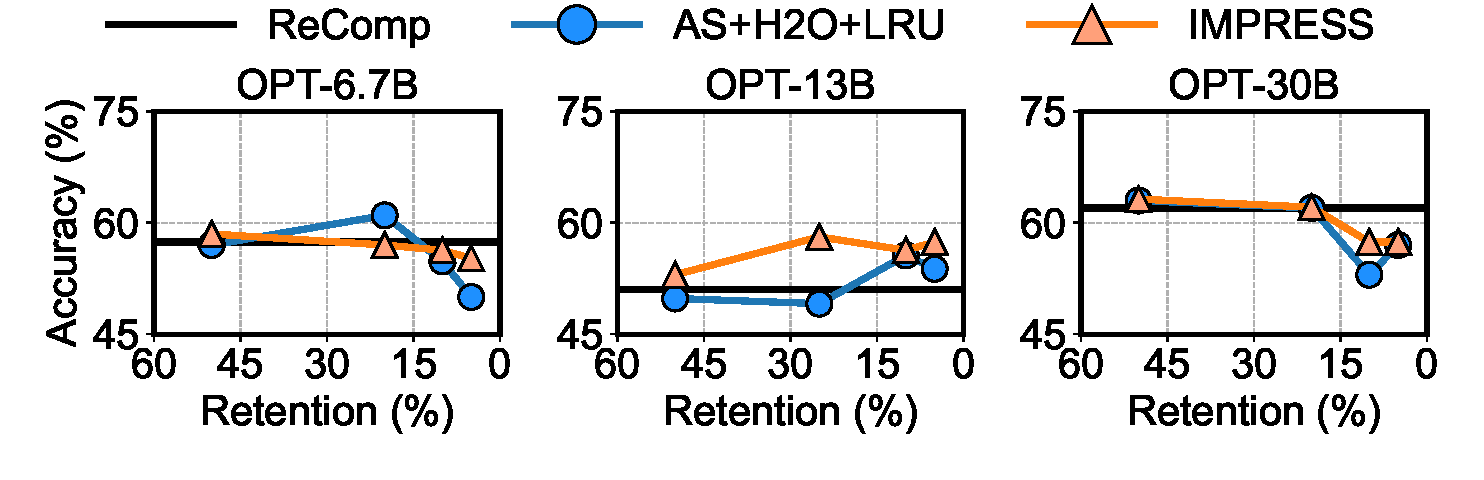
\includegraphics[width=3.3in, height=1.1in]{overall_acc1_rte.pdf}
	}
	\subfigure[COPA]{
		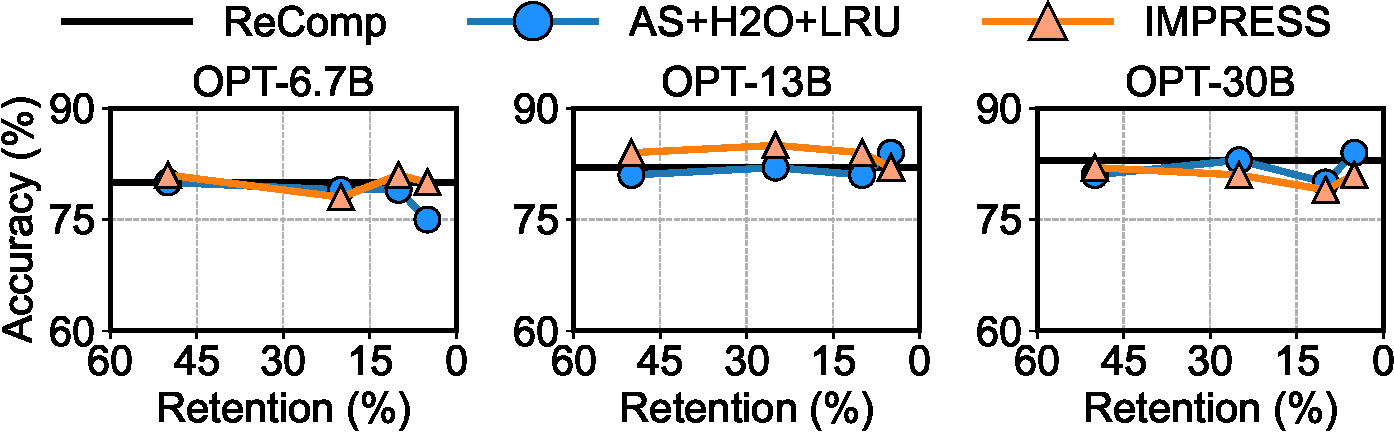
\includegraphics[width=3.3in, height=1.1in]{overall_acc1_copa.pdf}
	}
	\hspace{0.2in}
	\subfigure[OpenBookQA]{
		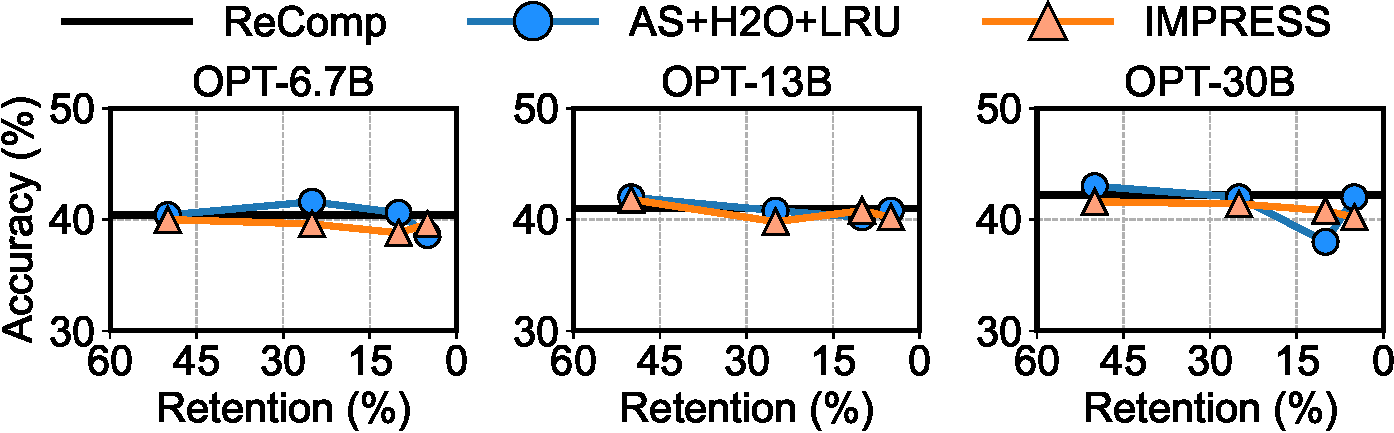
\includegraphics[width=3.3in, height=1.1in]{overall_acc1_openbookqa.pdf}
	}
	
	\vspace{-0.1in}
	\caption{
		Model generation quality of various systems across four datasets and three models.}
	\label{fig:overall_acc}
	\vspace{-0.1in}
\end{figure*}

%\noindent \textbf{Dual-cache replacement algorithm.} 
%The \pname{} system includes both GPU and CPU caches, each managed by different cache eviction strategies due to the varying granularity of data transfers from disk and CPU. Specifically, to optimize disk I/O efficiency, data is transferred from disk to CPU cache in chunks, regardless of the ratio of important KVs within each chunk. Consequently, the CPU cache eviction is only based on chunk access frequency to minimize the number of chunks loaded from the disk. 
%In contrast, when transferring data from the CPU cache to the GPU cache, only important KVs are transmitted to reduce  \ysl{the pressure on the PCIe bus}~\cite{flexgen-icml23}. Therefore, the \techbb{} method is employed in GPU cache eviction to minimize the transmission of important KVs.
%
%To achieve this, 
%we maintain two separate min-heaps in the GPU and CPU caches to assist with cache eviction. The top elements in the GPU heap are chunks with the lowest scores, while in the CPU heap, they are chunks with the lowest access frequency.
%When a new request arrives, the system first checks the radix tree-based meta data to identify reusable stored prefix KV chunks and locate whether they are located in the GPU cache, CPU cache, or disk.
%If the target chunk is in the GPU cache, after the chunk is accessed and its score is updated, it remains in the GPU cache.
%If the target chunk is in the CPU cache, its score is updated and compared with the smallest score in the GPU cache. If the target chunk's score is higher, it is swapped with the lowest-score chunk in the GPU cache; otherwise, it stays in the CPU cache.
%If the target chunk is on the disk, its access frequency is updated and compared with the lowest access frequency in the CPU cache. If the target chunk has a higher access frequency, it replaces the least-accessed chunk in the CPU; otherwise, it stays in the disk.

\noindent \textbf{Dual-cache replacement algorithm.}
% We use \techbb{} to manage both GPU and CPU caches. To achieve this, we maintain two min-heaps in CPU memory for the chunks in GPU and CPU memory to assist with cache eviction. 
% The top elements in two heaps point to the chunks with the lowest scores in the GPU and CPU caches respectively. 
% %We ensure that chunks in the GPU and CPU caches are non-redundant to maximize the amount of cached data. Additionally, 
% We ensure that all chunks' replicas are kept on disk to avoid I/O latency when evicting chunks from the CPU to disk.
We employ score-based cache replacement policy to oversee GPU and CPU caches, utilizing two min-heaps in CPU memory to manage chunks in both caches and facilitate eviction. The heaps' tops indicate the lowest-scored chunks in the GPU and CPU caches, respectively. To optimize data caching, we ensure non-redundancy between the GPU and CPU caches. Additionally, we maintain all chunk replicas on disk, thus eliminating I/O latency when chunks are evicted from CPU to disk.

Upon receiving a new request, \pname{} first identifies reusable important tokens and locates their associated chunks. If the chunk is already in the GPU cache, \pname{} utilizes the key or value vectors for inference and updates the chunk's score, retaining it in the GPU cache. If the chunk is in the CPU cache, after transferring the vectors to the GPU, \pname{} updates and compares the chunk's score with the GPU cache's lowest. If superior, it replaces the lowest-scored chunk in the GPU cache; otherwise, it stays in the CPU cache.
Should the chunk reside on disk, \pname{} loads it into CPU cache, transfers the necessary vectors to the GPU, and updates the chunk's score. This new score is then assessed against the lowest scores in both caches to decide whether the chunk should be promoted to the GPU cache, remain in the CPU cache, or stay on disk.



%\subsubsection{\techBb{}}
%当要读取的重要token的key or value vector在disk上时,\pname{} 首先会从disk加载其所在的chunk到CPU中,然后读取仅传送重要的key or value vectors 到GPU中从而减小PCIe传输量,最后决定该chunk是否被GPU或CPU缓存以备后续使用。
%However, we observed that the number of important key or value vectors in a chunk does not correlate with the chunk’s access frequency, as shown in Figure~\ref{fig:imp_token_num}. Therefore, existing systems that determine whether to cache a chunk in GPU memory or CPU memory based solely on access recency or frequency may reduce the hit ratio of important key-value pairs in the GPU cache, leading to an increase in data transferred via PCIe.
%
%To address this, we propose an importance-informed \techbb{} that further improves the GPU cache hit ratio and reduce the data transfer volume from CPU to GPU.
%The core idea is to assign a score to each chunk and use the score to determine whether it should be cached. 
%This score is defined as the cumulative number of important vectors accessed within each chunk.
%as its access frequency multiplied by the ratio of important keys or values it contains. 
%The chunks with higher scores are prioritized for caching in GPU memory, while those with lower scores are placed in CPU memory. 
%The score is updated after each chunk access.
% The ratio of important keys or values is computed as the moving average between two consecutive accesses and updated online after each chunk access.
%
%假设有三个chunk的访问频率分别是8, 10, 7;其中重要的token的数量分别是3, 1, 2。假设GPU和CPU都只能存储1个chunk,新的一些请求分别要访问8、10、7次三个chunk以获取其中重要的token用于推理。
%传统方法使用LFU缓存时会根据chunk访问频率从高到底放置如图x。那么传统方法一共需要经过PCIe传输8*3 + 7*2 = 38个vector。
%使用\techbb{}后,由于chunk1的score大于chunk2的score,因此放置如图x;那么一共需要经过PCIe传输10*1 + 7*2 = 24个vector。


